\documentclass[]{article}
\usepackage[T1]{fontenc}
\usepackage[utf8]{inputenc}
%\usepackage[icelandic]{babel}
\usepackage{caption}
\usepackage{circuitikz}
\usepackage{grffile} 
\usepackage[margin=1in]{geometry}
\usepackage{listings}

% grffile er pakki sem leifir manni að nota "" til þess að forðast að nota
% nafnið á myndinni með.
\usepackage{graphicx}
% \graphicspath{{images/}} Sýnir undir möppu þar sem myndirnar eru

\usepackage{hyperref}
%fyrirlinka - \url{www.....}
\begin{document}
\title{Þýðendur \\
	Verkefni 2\\
	Pétur Daníel Ámundason\\
	}
\maketitle

\section*{1.}
\subsection*{a)}
$E \rightarrow$ EE+ | EE* | t \\
Sýnið hvernig framleiða má strenginn tt+t* með þessari mállýsingu \\
Svar: $E => EE* => EE+E* => tE+E* => tt+E* => tt+t*$ \\

\subsection*{b)}
Sýnið þáttunartré fyrir þennan streng\\
Svar: \\

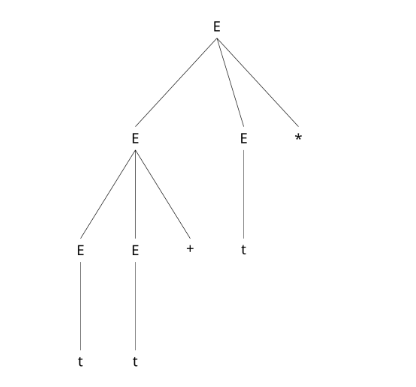
\includegraphics[scale=0.5]{tree}

\subsection*{c)}
Hvaða mál er framleitt af þessari mállýsingu. \\
Svar: Reiknisegð eftirrithætti (posix) og tvíundaraðgerðum + og *. Nota táknið t til þess að standa fyrir breytu.

\section*{5.}

\subsection*{a)}
Svar:\\
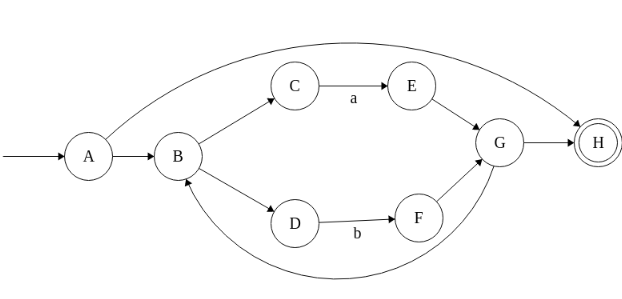
\includegraphics[scale=0.7]{NFAa}

\subsection*{b)}
Svar: \\
\includegraphics*[scale=0.6]{NFAb}

\subsection*{c)}
Svar: \\
\includegraphics*[scale=0.6]{NFAc}

\subsection*{d)}
Svar: \\
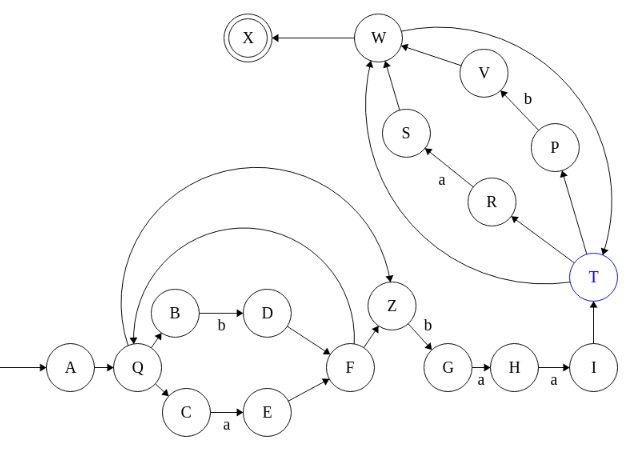
\includegraphics[scale=0.6]{NFAd}







\end{document}